\documentclass[12pt]{article}
\UseRawInputEncoding
\usepackage{tipa}
\usepackage{natbib}
\usepackage{graphicx}
\usepackage[normalem]{ulem}
%\useunder{\uline}{\ul}{}
\usepackage{qtree}
\usepackage{linguex}
\usepackage{booktabs}
\usepackage[table,xcdraw]{xcolor}
\usepackage{float}
\usepackage[margin=2.35cm]{geometry}
\usepackage{mathptmx}
\usepackage{setspace}
\usepackage[none]{hyphenat}
\usepackage{titlesec}
\usepackage{adjustbox}
\usepackage{tikz}
\usepackage{tikz-qtree}
\usepackage{float}
\usepackage{fancyvrb}
\usepackage{hyperref}
\usepackage{multicol}
%\usepackage{wrapfig}
%\usepackage[utf8]{inputenc}

\hypersetup{
  colorlinks   = true, %Colours links instead of ugly boxes
  urlcolor     = blue, %Colour for external hyperlinks
  linkcolor    = black, %Colour of internal links
  citecolor   = black %Colour of citations
}


% \graphicspath{ {images/} }
% \bibstyle{apa}
%\setcitestyle{aysep={}} 
%\setcitestyle{notesep={: }}
%\newcommand\cites[1]{\citeauthor{#1}'s\ (\citeyear{#1})}

%\bibliographystyle{apalike}


\usepackage{fancyhdr}
 
\pagestyle{fancy}
\fancyhf{}
\renewcommand{\headrulewidth}{0pt}
\rfoot{\thepage}

\renewcommand{\baselinestretch}{1}

\usepackage{lipsum}

\newcommand\blfootnote[1]{%
\begingroup
\renewcommand\thefootnote{}\footnote{#1}%
\addtocounter{footnote}{-1}%
\endgroup}

%\titlespacing\section{0pt}{12pt plus 4pt minus 2pt}{0pt plus 2pt minus 2pt}

\begin{document}
\setstretch{1.1}
\section*{\fontsize{16}{12}\selectfont Topicalization is (Still) Disappearing: \\\fontsize{14}{12}\selectfont information uniformity as a dimension of specialization}
 \noindent \fontsize{12}{12}\selectfont Joel C. Wallenberg, \textit{University of York}\\
\\
\noindent This article presents new data on the decline of DP ``topicalization'' (i.e. object fronting) in Late Early Modern English and its implications for the hypothesis that speakers prefer informational uniformity in their utterances \citep[][\textsl{inter alia}]{fenkfenk1980,fenk1989,fenk2001, levy2005,levyjaeger2007}. This study applies the version of the hypothesis in \citet{cuskleyetal2021}, that speakers distribute the information content of words as uniformly as possible across an entire utterance, to help explain the statistical patterns of syntactic change over long periods of time \citep[in a similar way to][]{wallenbergetal2021}. In particular, I will show that the topicalization of direct objects in English has declined since the Late Early Modern English period into the modern period, a pattern which is itself a continuation of the decline observed by \citet{speyer2008, speyer2010} in Middle English and Early Modern English. Furthermore, the decline persists even though the topicalization and non-topicalization orders are functionally differentiated (i.e. specialized) for different \\informational and prosodic contexts.\\

\noindent \citet{speyer2008,speyer2010} showed that the frequency of direct object topicalization, and fronting of other constituents, declined during much of the history of English. He also tied this to a particular prosodic effect: the desire of speakers to avoid a stress clash between the subject and the fronted constituent. He showed observationally and experimentally that topicalization sentences such as \ref{clash} below, in which a prosodically strong/heavy nominal object appears next to a similar nominal subject were dispreferred compared to topicalizations in which the subject was a pronoun, as in \ref{pron}, and \textsl{in situ} sentences \ref{insitu}.


\ex. \label{exs}
\a. \label{clash} The cat Mary likes.
\b. \label{pron}	The cat she likes.

\ex. \label{insitu} Mary/she likes the cat.\\ 

\noindent Speyer further convincingly argued that the avoidance of \ref{clash} is due to prosodic clash between object and subject, showing that experimental participants insert a pause between the two if they are required to produce sentences like \ref{clash}. He then explained the decline in topicalization over the history of English as a consequence of the decline of verb-second (V2) orders, which allowed for a prosodically weaker verb to intervene between object and subject in sentences with fronting (as occurs in all the modern Germanic languages other than English). Note also that the same strategies which prevent the prosodic clash \textsl{also} prevent a peak of high information item (i.e. lower frequency words and phrases) at the beginning of a clause. However, even though topicalization and \textsl{in situ} object orders could be considered specialized for clash and non-clash contexts, this description does not explain why they still overlap in function \cite{prince1998}. \\

\noindent I explore the hypothesis that, in addition to prosodic context, the use of the orders also depends on the degree of information uniformity each one allows a speaker to achieve in an utterance (as measured by the ``Deviation of the Rolling Mean'' (DORM) of a sentence's ordered information content (surprisal) values, cf. \citealt{cuskleyetal2021, wallenbergetal2021}). Because degree of uniformity is a continuous dimension, the two syntactic variants cannot specialize completely along it \citep{wallenberg2016, wallenberg2019}; they therefore still overlap in their functions, and so compete in use \cite{kroch1994}. The current study uses the \textsl{Penn Parsed Corpus of Early Modern English} and \textsl{Penn Parsed Corpus of Modern British English 2} \citep[PPCEME, PPCMBE2;][]{ppceme, ppcmbe2}, and finds two results confirming the incomplete specialization hypothesis: first, the decline in topicalization continued after the period in which V2 orders were lost, and secondly, the decline persists in clearly non-V2 sentences, even where the subject is a pronoun (see Figure \ref{decline}). \\

\begin{figure}
\centering
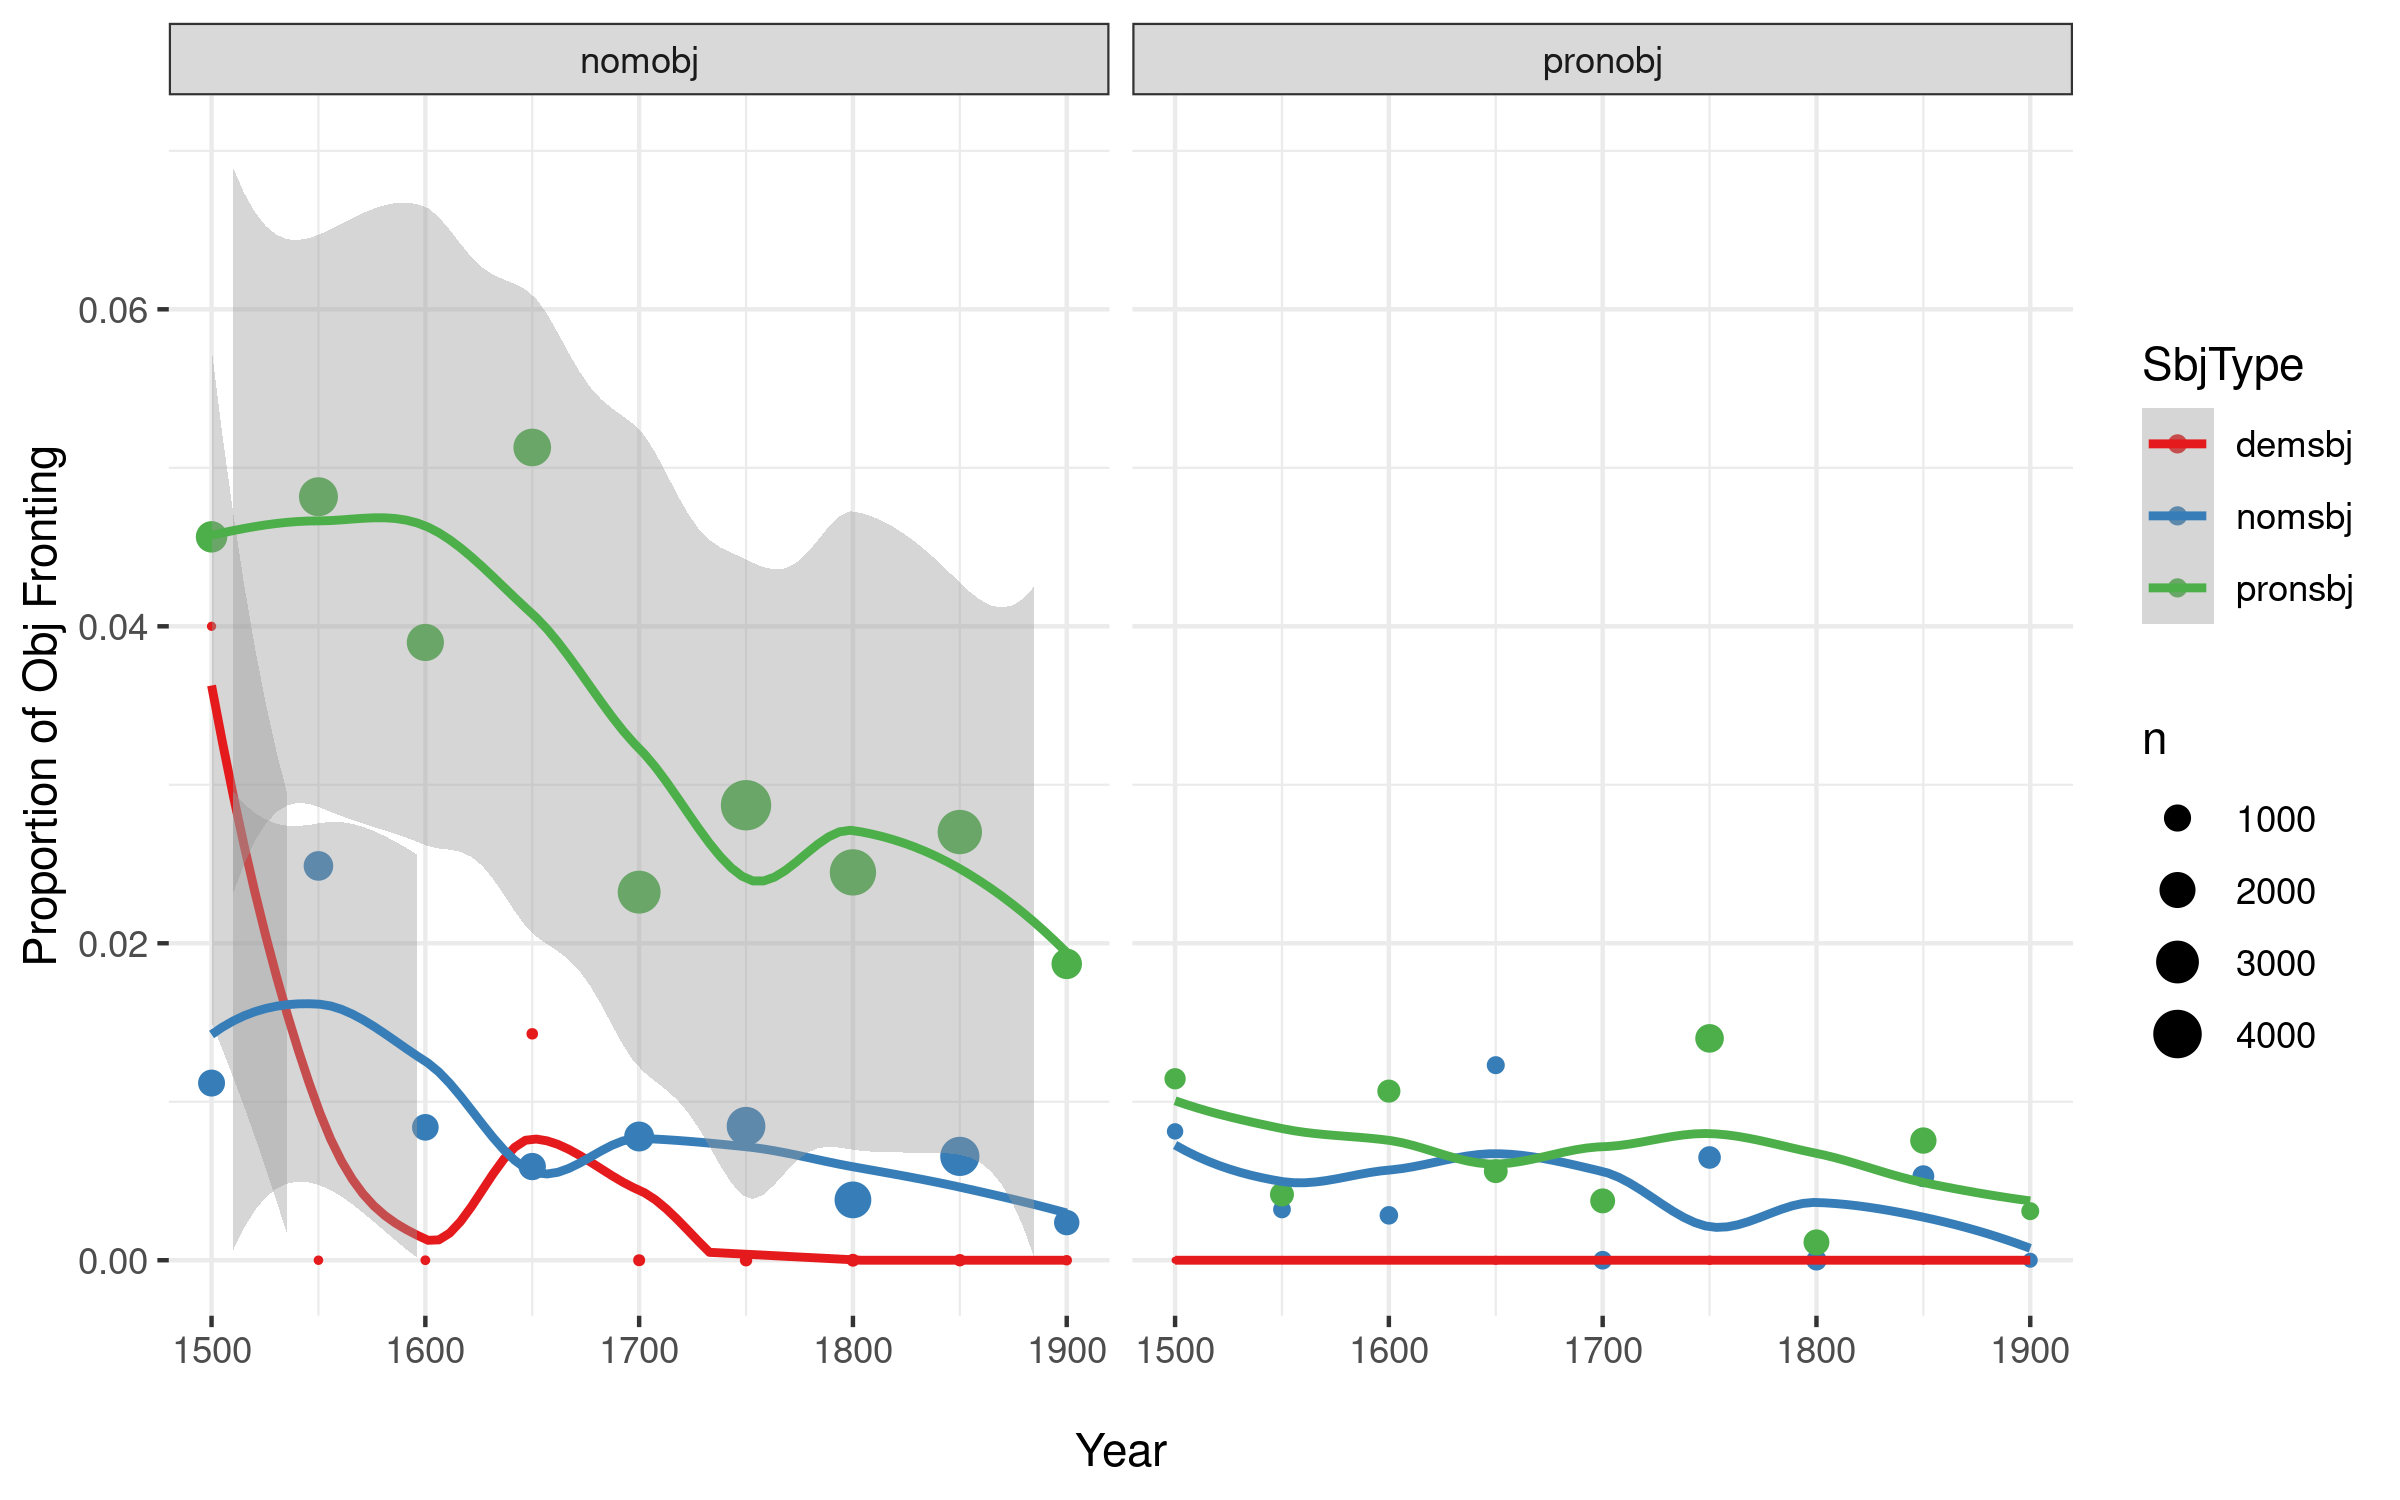
\includegraphics[scale=0.75]{objTop.png}
\caption{\small{Decline of direct object DP fronting in Early Modern and Modern British English, as measured in the PPCEME and PPCMBE2 (\~ 4.5 million words from 1500 to 1920), faceted by object type (nominal vs pronominal and subject type (demonstrative, nominal, or pronominal).}}
\label{decline}
\end{figure}

\noindent This continued competition between the variants and consequent diachronic decline of one variant, even though it has slowed \citep[as predicted in][]{wallenberg2016}, is entirely what one would expect if the variants cannot completely differentiate in their contexts of use. The full article will go further in relating the speed of decline to the information uniformity DORM measures of the relevant populations of sentences.

\vspace{-0.1em}

\begin{multicols}{2}
\noindent \textbf{References}
\vspace{-0.28em}
\renewcommand{\section}[2]{}
\bibliographystyle{linquiry2}
\setlength{\bibsep}{0.0pt}
\bibliography{joelrefs}
\end{multicols}

\end{document}